\section{Codificação das instruções}
	Instrução é uma palavra da linguagem de máquina, sua codificação é de fundamental importância para o processamento das operações.	Todas as instruções contém 32 bits. Exitem 4 formatos de instruções: R (R-type), I (I-type), Load/Store e Jump. Os OPCODES são os códigos de operação da instrução, neste documento ele é representação em números hexadecimais.\\
	
  \FloatBarrier
    \begin{center}
\begin{longtable}[pos]{| c | c | c | m{7cm} |} \hline    
          \multicolumn{1}{|c|}{\cellcolor[gray]{0.9}\textbf{Formato da instrução}} & 
          \multicolumn{1}{c|}{\cellcolor[gray]{0.9}\textbf{Instrução}} & 
          \multicolumn{1}{c|}{\cellcolor[gray]{0.9}\textbf{Descrição}} \\ \hline
          \endfirsthead
          \hline
          \multicolumn{3}{|l|}
          {{\bfseries continuação da página anterior}} \\
          \hline
          \multicolumn{1}{|c|}{\cellcolor[gray]{0.9}\textbf{Formato da Instrução}} & 
          \multicolumn{1}{c|}{\cellcolor[gray]{0.9}\textbf{Instrução}} & 
          \multicolumn{1}{c|}{\cellcolor[gray]{0.9}\textbf{Descrição}} \\ \hline
          \endhead

          \multicolumn{3}{|r|}{{continua na próxima página}} \\ \hline
          \endfoot

          \hline
          \endlastfoot 
           
			\multirow{8}{*}{R-type} & ADD & Soma dois valores \\ \cline{2-3}	
	& SUB & Subtrai dois valores \\ \cline{2-3}	
	& MUL & Multiplica dois valores \\ \cline{2-3}	
	& DIV & Divide dois valores \\ \cline{2-3}
	& AND & AND lógico \\ \cline{2-3}
	& OR & OR lógico  \\ \cline{2-3}
	& CMP & Compara dois valores \\ \cline{2-3}
	& NOT & NOT lógico \\ \hline 
	\multirow{4}{*}{I-type} & ADDI & Soma dois valores,um destes imediato. \\ \cline{2-3}
	& SUBI & Subtrai dois valores, um destes imediato. \\ \cline{2-3}
	& ANDI & AND lógico de dois valores, um destes imediato. \\ \cline{2-3}
	& ORI & OR lógico de dois valores, um destes imediato. \\ \cline{2-3}
	& LW & Leitura de um dado da memória de dados \\ \cline{2-3}
	& SW & Armazena um dado na memória de dados \\ \hline
	\multirow{6}{*}{Jump} & JP & Desvia para um destino \\ \cline{2-3}
	& JPC & Desvia para um destino relativo ao PC \\ \cline{2-3}
	& BRFL & Desvia para um destino se RF==CST \\ \cline{2-3}
	& CALL & Chamada de subrotina \\ \cline{2-3}
	& RET & Retorno de Subrotina \\ \cline{2-3}
	& HALT & Parada do sistema \\ \cline{2-3}
	& NOPE & Refresh no módulo \\ \hline
\end{longtable}
\end{center}


	O formato R está relacionado as instruções lógicas e aritméticas.
	\begin{figure}[H]
    	\centering
    	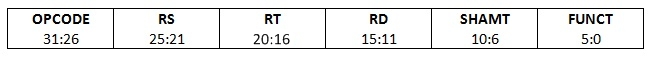
\includegraphics{r-format}
    	\caption{Formato R}
		\label{r_format}
	\end{figure}
	Seus respectivos campos são:
	\begin{itemize}
	\item \textbf{OPCODE} - Código da operação básica da instrução.
	\item \textbf{RS} - Registrador do primeiro operando de origem.
	\item \textbf{RT} - Registrador do segundo operando de origem.
	\item \textbf{RD} - Registrador destino.
	\item \textbf{SHAMT} - \textit{Shift amount}; Quantidade de deslocamento.
	\item \textbf{FUNCT} - Função; Esse campo seleciona a variante específica da operação no campo opcode, e as vezes, é chamado de código de função.
\end{itemize}	

\begin{table}[H]
\centering
	\begin{tabular}{|c|c|c|}
  	\hline 
  	\cellcolor[gray]{0.9}\textbf{OPCODE} & \cellcolor[gray]{0.9}\textbf{INSTRUCTION} & \cellcolor[gray]{0.9}\textbf{FUNCTION} \\ 
  	\hline 
  	0x00 & ADD & 0x20 \\ 
  	\hline 
  	0x00 & SUB & 0x20 \\ 
  	\hline 
  	0x00 & MUL & 0x18 \\ 
  	\hline 
  	0x00 & DIV & 0x1A \\ 
  	\hline 
  	0x00 & AND & 0x24 \\ 
  	\hline 
  	0x00 & OR & 0x25 \\ 
  	\hline 
  	0x00 & CMP & 0x1C \\ 
  	\hline 
  	0x00 & NOT & 0x1D \\ 
  	\hline 
  	\end{tabular} 
  	\caption{Definição dos OPCODES do formato R}
  \end{table} 
  	 	
  	
	 Um segundo tipo de formato de instrução é chamado de formato I, utilizado pelas instruções imediatas e de transferência de dados.
	\begin{figure}[H]
    	\centering
    	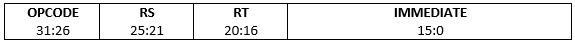
\includegraphics{i-format}
    	\caption{Formato I}
		\label{i_format}
  	\end{figure}
Seus respectivos campos são:
	\begin{itemize}
	\item \textbf{OPCODE} - Código da operação básica da instrução.
	\item \textbf{RS} - Registrador do operando de origem.
	\item \textbf{RT} - Registrador destino.
	\item \textbf{ADDRESS OR IMMEDIATE} - Endereço de memória ou constante numérica.
\end{itemize}	  	

\begin{table}[H]
\centering	
\begin{tabular}{|c|c|}
	\hline 
  	\cellcolor[gray]{0.9}\textbf{OPCODE} & \cellcolor[gray]{0.9}\textbf{INSTRUCTION} \\ 
	\hline 
	0x08 & ADDI \\ %
	\hline 
	0x10 & SUBI \\ %
	\hline 
	0x0c & ANDI \\ %
	\hline 
	0x13 & ORI \\ %
	\hline 
	0x23 & LW \\ %
	\hline 
	0x2b & SW \\ %	
%	0x2a
%0x04
%0x04
	\hline 
	\end{tabular} 
	  	\caption{Definição dos OPCODES do formato I}	
\end{table}	
	
 O formato Jump servem para as instruções de desvio incondicional.  	
   	\begin{figure}[H]
    	\centering
    	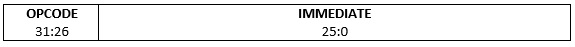
\includegraphics{jump}
    	\caption{Formato Jump}
		\label{jump}
  	\end{figure}
Seus respectivos campos são:
	\begin{itemize}
	\item \textbf{OPCODE} - Código da operação básica da instrução.
	\item \textbf{ADDRESS} - Endereço de memória ou constante numérica.
\end{itemize}
 
\begin{table}[H]
\centering 	
  	\begin{tabular}{|c|c|}
  	\hline 
  	\cellcolor[gray]{0.9}\textbf{OPCODE} & \cellcolor[gray]{0.9}\textbf{INSTRUCTION} \\ 
  	\hline 
  	09 & JP \\ 
  	\hline 
  	0A & JPC \\ 
  	\hline 
  	0x09 & BRFL \\ 
  	\hline 
  	0C & CALL \\ 
  	\hline 
  	0D & RET \\ 
  	\hline 
  	0E & HALT \\ 
  	\hline 
  	00 & NOPE \\ 
  	\hline 
  	\end{tabular} 
  	  	\caption{Definição dos OPCODES do formato Jump}
\end{table}